\documentclass[12pt, titlepage]{article}

\usepackage{booktabs}
\usepackage{tabularx}
\usepackage{hyperref}
\hypersetup{
    colorlinks,
    citecolor=black,
    filecolor=black,
    linkcolor=red,
    urlcolor=blue
}
\usepackage[round]{natbib}
\usepackage{booktabs}

\usepackage{amsmath, mathtools}
\usepackage{amsfonts}
\usepackage{amssymb}
\usepackage{graphicx}
\usepackage{colortbl}
\usepackage{xr}
\usepackage{hyperref}
\usepackage{longtable}
\usepackage{xfrac}
\usepackage{tabularx}
\usepackage{float}
\usepackage{siunitx}
\usepackage{booktabs}
\usepackage{pdflscape}
\usepackage{afterpage}
\usepackage{float}
\usepackage{fancyvrb}
\usepackage{lscape}
\usepackage{relsize}
\usepackage{listings}
\usepackage{caption}
\usepackage{subcaption}
\usepackage[round]{natbib}
\newcommand{\tref}[1]{T\ref{#1}}
\title{FFT Library}

\author{
Yuzhi Zhao\\
}

\date{\today}

%% Comments

\usepackage{color}

\newif\ifcomments\commentstrue

\ifcomments
\newcommand{\authornote}[3]{\textcolor{#1}{[#3 ---#2]}}
\newcommand{\todo}[1]{\textcolor{red}{[TODO: #1]}}
\else
\newcommand{\authornote}[3]{}
\newcommand{\todo}[1]{}
\fi

\newcommand{\wss}[1]{\authornote{blue}{SS}{#1}}
\newcommand{\an}[1]{\authornote{magenta}{Author}{#1}}
\newcommand{\wss}[1]{\authornote{blue}{SS}{#1}}



\begin{document}

\maketitle

\pagenumbering{roman}
\tableofcontents
\listoftables
\listoffigures

\begin{table}[bp]
\caption{\bf Revision History}
\begin{tabularx}{\textwidth}{p{3cm}p{2cm}X}
\toprule {\bf Date} & {\bf Version} & {\bf Notes}\\
\midrule
Date 1 & 1.0 & Notes\\
Date 2 & 1.1 & Notes\\
\bottomrule
\end{tabularx}
\end{table}

\newpage

\pagenumbering{arabic}

This document ...

\section{Functional Requirements Evaluation}
Please reference TestPlan System Test Description Section \url{https://github.com/741ProjectFFT/FFT/tree/master/Doc/TestPlan}.\\\\
Test Guide for all system tests below:\\
\begin{figure}[H]
 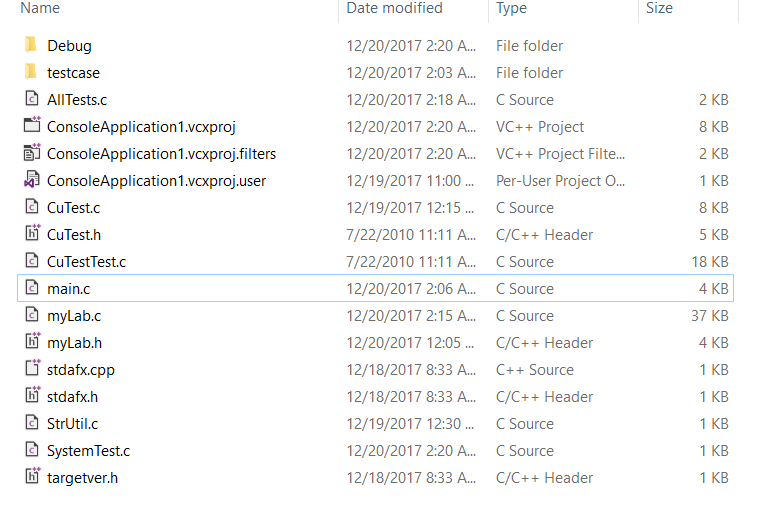
\includegraphics[width=\linewidth]{directory.PNG}
  \caption{program files directory layout}
  \label{fig:Direc}
\end{figure}
Step1: Be aware that when we want to do system test we should add all .h files and .c files into the project.\\
Step2: Remove the SystemTest.c and ALLTEST.c from the project not deleting them.\\
Step3: Run each block once a time.
Step4: Then remove the main.c from the project and add SystemTest.c into this project.\\
Step5: Open SystemTest.c file and change the file name every time when we want to test each test cases' results.\\
Because we already run the main function for each block so that we got all output files with a corresponding name.\\
Files with name called "test*\_out.txt" is the output for "test*.txt" from matlab. And "test*\_real.txt" is the output file from this 
FFT library. Thus, the file name should be changed every time with a pair  "test*\_out.txt" and "test*\_real.txt" and * should be the same number.\\
Step6: Run SystemTest.c, the window will show the MSE value.

\subsection {T-1 Radix-2 Complex Number FFT Calculation Function (T 1)}
Test input numbers in "test1.txt".  The result is shown below:\\
\begin{figure}[H]
 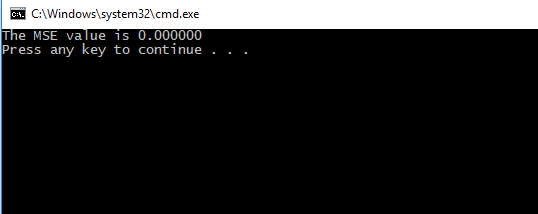
\includegraphics[width=\linewidth]{t1.PNG}
  \caption{result from T-1}
  \label{fig:T1}
\end{figure}
MSE = 0.000000 means that the results from Matlab and this FFT library are nearly the same and the system test passed.

\subsection {T-2 Radix-2 Real Number Calculation Function   (T 2)}
Test input numbers in "test2.txt".  The result is shown below:\\
\begin{figure}[H]
 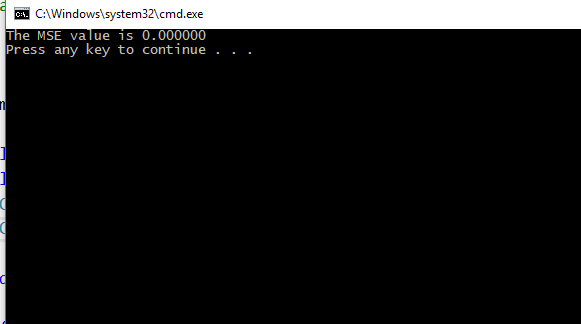
\includegraphics[width=\linewidth]{t2.PNG}
  \caption{result from T-2}
  \label{fig:T2}
\end{figure}
MSE = 0.000000 means that the results from Matlab and this FFT library are nearly the same and the system test passed.


\subsection {T-3 Radix-2 Complex Number IFFT Calculation Function (T 3)}
Test input numbers in "test1.txt".  The result is shown below:\\
\begin{figure}[H]
 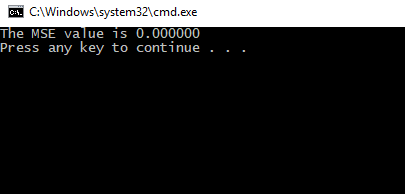
\includegraphics[width=\linewidth]{t3.PNG}
  \caption{result from T-3}
  \label{fig:T3}
\end{figure}
MSE = 0.000000 means that the results from Matlab and this FFT library are nearly the same and the system test passed.

\subsection {T-4 Radix-2 Real Number IFFT Calculation Function  (T 4)}
Test input numbers in "test4.txt".  The result is shown below:\\
\begin{figure}[H]
 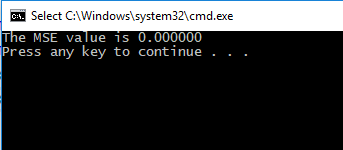
\includegraphics[width=\linewidth]{t4.PNG}
  \caption{result from T-4}
  \label{fig:T4}
\end{figure}
MSE = 0.000000 means that the results from Matlab and this FFT library are nearly the same and the system test passed.



\subsection {T-5 Radix-3 Complex Number FFT Calculation Function  (T 5)}
Test input numbers in "test5.txt".  \\
Not implemented successfully.
\subsection {T-3 Radix-2 Complex Number IFFT Calculation Function  (T 6)}
Test input numbers in "test6.txt". \\
Not implemented successfully.
\subsection {T-3 Radix-2 Complex Number IFFT Calculation Function (T 7)}
Test input numbers in "test7.txt".  \\
Not implemented successfully.
\subsection {T-3 Radix-2 Complex Number IFFT Calculation Function (T 8)}
Test input numbers in "test8.txt". \\
Not implemented successfully.

\section{Nonfunctional Requirements Evaluation}
\subsection{Usability}
		
\subsection{Performance}

\subsection{etc.}
	
\section{Comparison to Existing Implementation}	

Compare with FFT Library in Matlab(T 9)
\begin{figure}[H]
 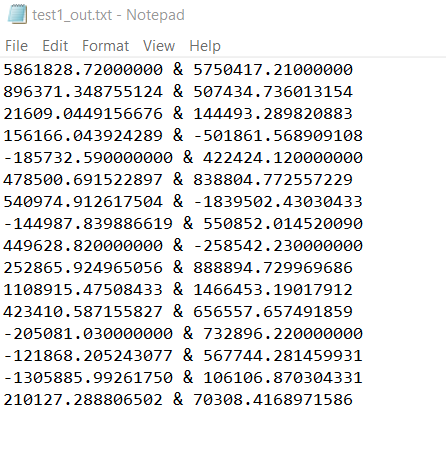
\includegraphics[width=\linewidth]{p1.PNG}
  \caption{result from test1\_out.text}
  \label{fig:T4}
\end{figure}\begin{figure}[H]
 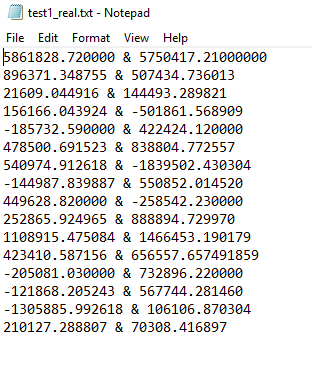
\includegraphics[width=\linewidth]{p2.PNG}
  \caption{result from  test1\_real.text}
  \label{fig:T4}
\end{figure}
As the output values from Matlab and this FFT library, the precision of the numbers are different. So this library can be further improved to achieve better precision.

\section{Unit Testing}
Test guide:\\
Remove main.c and SystemTest.c from project and add ALLTEST.c to project and run it, the result will be shown below:\\
\begin{figure}[H]
 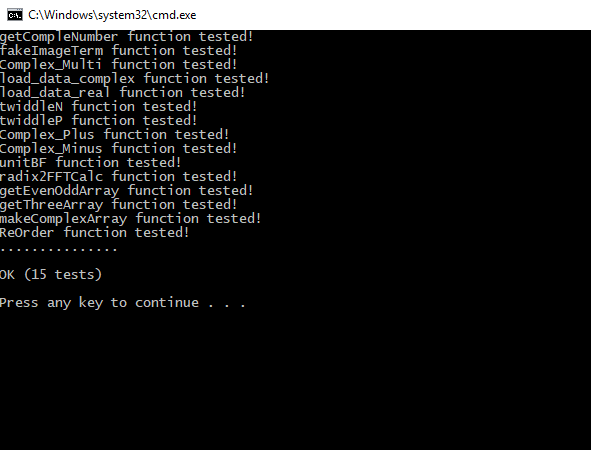
\includegraphics[width=\linewidth]{test.PNG}
  \caption{result from Test}
  \label{fig:Test}
\end{figure}
Detailed unit test case including inputs and outputs information was described in TestPlan unit test section. Reference \url{https://github.com/741ProjectFFT/FFT/tree/master/Doc/TestPlan}

\section{Changes Due to Testing}
\begin{itemize}	
	\item Because of adding system test and unit test, the whole project will have totally three main functions. And they can not be run even can not exits in the project at the same time.
	\item  myLab.c file was added more functions used to do unit test.
	\item CuTest.h and CuTest.h files should be included in th project.

\end{itemize}	

\section{Automated Testing}
If consider the system test and unit test as independent test behaviors,  unit test is fully automated. For system test, it was done by manually and automated half to half since we have to 
manually add files and remove files from our project. Also the test file name have to be modified manually.		
\section{Trace to Requirements}
\begin{table} [H]
  \caption{Requirements Traceability Matrix}
  \label{Table:Table_Traceability_CA}  
\begin{tabular}{|c|p{8cm}|}
  \hline	
  \textbf{Test Number} & \textbf{CA Instance Model}\\
  \hline 
   T1& IM1\\ \hline
   T2& IM1\\ \hline
   T3& IM1\\ \hline
   T4& IM1\\ \hline
   T5& IM2\\ \hline
   T6& IM2\\ \hline
   T7& IM2\\ \hline
   T8& IM2\\ \hline
   T9& IM1, IM2\\ \hline
   T10& IM1, IM2\\ \hline

\end{tabular}\\
\end{table}
Due to differences between CA and SRS template. There is no specific requirement stated in CA. So here only map test number to CA Instance models.		
\section{Trace to Modules}		
\begin{table} [H]
  \caption{Model Traceability Matrix}
  \label{Table:Table_Traceability_MG}  
\begin{tabular}{|c|p{8cm}|}
  \hline	
  \textbf{Test Number} & \textbf{CA Instance Model}\\
  \hline 
   T1& M1, M2, M3\\ \hline
   T2&  M1, M2, M3\\ \hline
   T3& M1, M2, M3\\ \hline
   T4& M1, M2, M3\\ \hline
   T5& M1, M2, M3\\ \hline
   T6& M1, M2, M3\\ \hline
   T7& M1, M2, M3\\ \hline
   T8&  M1, M2, M3\\ \hline
   T9& M1, M2, M3\\ \hline
   T10& M1, M2, M3\\ \hline

\end{tabular}\\
\end{table}
M1 reference Input Module;\\
M2 reference FFT Calculation Module;\\
M1 reference Output Module;\\

\section{Code Coverage Metrics}
N/A
\bibliographystyle{plainnat}

\bibliography{SRS}

\end{document}